\documentclass[compress]{beamer}

\usepackage[utf8]{vntex}
\usepackage{longtable}
\usepackage{amsmath}
\usepackage{amsmath}
\usepackage{amsfonts}
\usepackage{amssymb}
\usepackage[utf8]{inputenc}
\usepackage[absolute,overlay]{textpos}

\usepackage{listings}
\lstset{
	language = Java,
	frame = single,
	tabsize = 3
}

\usetheme{Warsaw}
%\usetheme{Antibes}
%\usecolortheme{spruce}
%\setbeamercolor{structure}{fg=cyan!90!blue}

\expandafter\def\expandafter\insertshorttitle\expandafter{%
    \insertshorttitle\hfill%
    \insertframenumber\,/\,\inserttotalframenumber}
      
\AtBeginSection[] % Do nothing for \section*
{
\begin{frame}
\tableofcontents[currentsection]
\end{frame}
}
\AtBeginSubsection[] % Do nothing for \section*
{
\begin{frame}
\tableofcontents[currentsection, currentsubsection]
\end{frame}
}

\title[]{Quản Trị Dự Án} 

\author[Bùi Đức Quang, Đặng Quang Trung, Nguyễn Văn Thuyên]{
Sinh viên thực hiện\\
Bùi Đức Quang - 20133067\\
Đặng Quang Trung - 20134145\\
Nguyễn Văn Thuyên - 20133847 \\[0.4cm]
Giảng viên \\
TS. Vũ Thị Hương Giang
}

\begin{document} 
\begin{frame}
\titlepage
\end{frame} 
  
\begin{frame}{Nội dung trình bày}
\tableofcontents
\end{frame}
\section{Request for proposal}
\begin{frame}{Request for proposal}
\begin{itemize}
\item[1. ] \textbf{Background of company}
\begin{itemize}
\item Công ty: BK-PM08
\item Mô tả: Công ty chuyên về outsourcing đưa ra các giải pháp xây dựng hệ thống liên quan đến thương mại điện tử.
\item Địa chỉ liên hệ: Số 1 Đại Cồ Việt, Đại học Bách Khoa Hà Nội.
\end{itemize}
\item[2. ] \textbf{Policy of proposal}
\begin{itemize}
\item Website phải thân thiện với người dùng (dễ sử dụng, bố cục web ưa nhìn, ...)
\item Website phải đảm bảo được việc luôn hoạt động 24/24 phục vụ cho khách mua hàng.
\item Tốc độ phản hồi cho người dùng nhanh chóng.
\item Có thể thanh toán trực tuyến (sử dụng thẻ visa card, master card, ...)
\item Người dùng có thể đăng nhập vào website thông qua tài khoản google, facebook, hoặc đăng ký tài khoản (sử dụng cho mua hàng hoặc tương tác bình luận về sản phẩm)
\item \ldots
\end{itemize}
\end{itemize}
\end{frame}
\begin{frame}{Request for proposal}
\begin{itemize}
\item[3. ] \textbf{Condition}
\begin{itemize}
\item Bên phía công ty ABCWear:
\begin{itemize}
\item Cung cấp đầy đủ cơ sở dữ liệu, máy chủ cho đội phát triển dự án.
\item Chịu trách nhiệm về hoàn thành thanh toán cho ngân sách dự án.
\item Hỗ trợ bên công ty BK-PM08 một số nghiệp vụ liên quan khi cần thiết.
\end{itemize}
\end{itemize}
\item[4. ] \textbf{Timeline}
\begin{itemize}
\item Thời hạn phát triển dự án là 3 tháng.
\item Sau khi hoàn thành dự án công ty BK-PM08 sẽ chịu trách nhiệm bảo trì sản phẩm 1 năm.
\end{itemize}
\item[5. ] \textbf{Estimate cost}
\begin{itemize}
\item Ước lượng chi phí dựa trên thời gian và mức độ phức tạp của chức năng
\end{itemize}
\end{itemize}
\end{frame}
\begin{frame}{Request for proposal}
\begin{itemize}
\item[6. ] \textbf{Schedule}
\begin{itemize}
\item Sử dụng 8\% ngày trong dự án cho các công việc:
\begin{itemize}
\item Phân tích yêu cầu khách hàng (các chức năng, ...)
\item Lập kế hoạch phát triển dự án.
\item Thuê các dịch vụ, công nghệ cần dùng trong dự án.
\end{itemize}
\item Sử dụng 12\% ngày trong dự án cho các công việc:
\begin{itemize}
\item Thiết kế hệ thống.
\item Xử lý các luồng hoạt động của website cho phù hợp với các điều kiện.
\end{itemize}
\item Sử dụng 50\% ngày trong dự án cho các công việc:
\begin{itemize}
\item Thực hiện việc cài đặt và kiểm thử hệ thống.
\item Đưa ra các bản demo cho khách hàng xem xét, tham khảo.
\end{itemize}
\item Sử dụng 10\% ngày còn lại:
\begin{itemize}
\item Test hệ thống thực.
\item Chạy hệ thống thực theo dõi, đánh giá và sửa chữa lỗi nếu có.
\end{itemize}
\end{itemize}
\end{itemize}
\end{frame}
\begin{frame}{Request for proposal}
\begin{itemize}
\item[7. ] \textbf{Meting}
\begin{itemize}
\item Đánh giá dự án theo các tiêu chí:
\begin{itemize}
\item Đánh giá theo tiến độ dự án.
\item Đánh giá theo chức năng hệ thống.
\end{itemize}
\end{itemize}
\item[8. ] \textbf{Condition of contract}
\begin{itemize}
\item Bên ABC wear:
\begin{itemize}
\item Đảm bảo thanh toán đầy đủ các khoản của dự án theo hợp đồng.
\item Đảm bảo cung cấp chính sách thông số và tài liệu kỹ thuật liên quan đến dự án.
\end{itemize}
\item Bên BK-PM08:
\begin{itemize}
\item Đảm bảo an toàn thông tin của bên công ty ABCwear.
\item Chịu trách nhiệm xây dựng hệ thống.
\item Cung cấp các tài liệu hướng dẫn sử dụng hệ thống, cũng như mã nguồn, tài liệu liên quan đến hệ thống cho công ty ABCwear khi cần.
\item Chịu trách nhiệm bảo trì cho hệ thống 1 năm sau khi kết thúc dự án.
\end{itemize}
\end{itemize}
\end{itemize}
\end{frame}
\section{Project Planning}
\subsection{Product / Project scope}
\begin{frame}{Product / Project scope}
\begin{itemize}
\item[1. ] \textbf{Business case/mission}
\begin{itemize}
\item Tiến độ: Thời gian hoàn thành dự án: 3 tháng 
\item Ngân quỹ: 300 triệu.
\item Giả định: Cung cấp đầy đủ cơ sở dữ liệu, máy chủ cho đội phát triển dự án
\end{itemize}
\item[2. ] \textbf{Project background and statement of need}
\begin{itemize}
\item Server
\item Client
\item Database
\end{itemize}
\item[3. ] \textbf{Goals and objectives}
\begin{itemize}
\item Mở rộng kinh doanh trực tuyến
\begin{itemize}
\item Cửa hàng quẩn áo.
\item Người mua hàng trực tuyến.
\end{itemize}
\item Hỗ trợ quán lí mua bán
\begin{itemize}
\item Chủ cửa hàng, nhân viên cửa hàng.
\end{itemize}
\end{itemize}
\end{itemize}
\end{frame}
\begin{frame}{Product / Project scope}
\begin{itemize}
\item[4. ] \textbf{Stakeholders}
\begin{itemize}
\item Vested Personnel
\begin{figure}[h]
\begin{center}
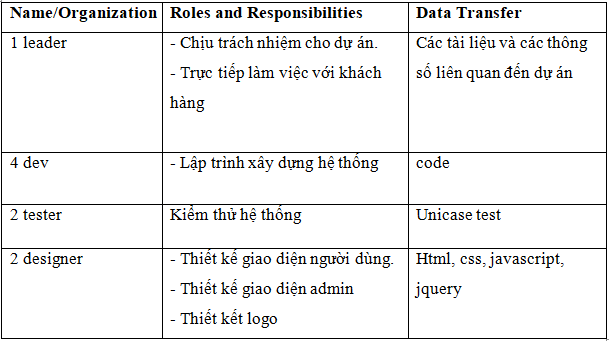
\includegraphics[scale=0.6]{QT.png}
\end{center}
\end{figure}
\end{itemize}
\end{itemize}
\end{frame}
\begin{frame}{Product / Project scope}
\begin{itemize}
\item[4. ] \textbf{Stakeholders}
\begin{itemize}
\item Influential Personnel
\begin{figure}[h]
\begin{center}
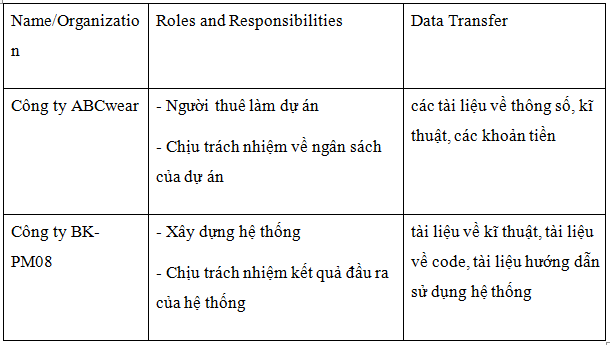
\includegraphics[scale=0.6]{QT1.png}
\end{center}
\end{figure}
\end{itemize}
\end{itemize}
\end{frame}
\begin{frame}{Product / Project scope}
\begin{itemize}
\item[5. ] \textbf{Driver, constraints, dependencies}
\begin{itemize}
\item Federal regulations:
\begin{itemize}
\item Công ty ABCwear là công ty đặt sản phẩm
\item Công ty BK-PM08 là công ty thực hiện xây dựng hệ thống
\end{itemize}
\item Standards
\begin{itemize}
\item Xây dựng trang web theo mô hình MVC
\end{itemize}
\item Exists systems/process
\begin{itemize}
\item Cơ sở dữ liệu có sẵn bao gồm các sản phẩm và khách hàng thường xuyên.
\end{itemize}
\item Schedules
\item Budgets
\begin{itemize}
\item Giai đoạn 1: Hoàn thành 20\% dự án: thanh toán 100 triệu đồng.
\item Giai đoạn 2: Hoàn thành 20\% dự án: thanh toán 100 triệu đồng.
\item Giai đoạn 3: Hoàn thành 100\% dự án: thanh toán số tiền còn lại.
\end{itemize}
\end{itemize}
\end{itemize}
\end{frame}
\begin{frame}{Product / Project scope}
\begin{itemize}
\item[6. ] \textbf{High-level operational concept (or use case)}
\begin{itemize}
\item Người quản trị
\begin{itemize}
\item Đăng nhập, đăng xuất
\item Thêm, sửa, xóa sản phẩm
\item \ldots
\end{itemize}
\item Người dùng
\begin{itemize}
\item Xem thông tin sản phẩm
\item Tìm kiếm sản phẩm
\item So sánh sản phẩm
\item \ldots
\end{itemize}
\end{itemize}
\item[7. ] \textbf{External interfaces}
\begin{itemize}
\item Xây dựng giao diện admin
\begin{itemize}
\item quản lý sản phẩm, tài khoản, doanh thu, đơn hàng.
\end{itemize}
\item Xây dựng giao diện người dùng
\begin{itemize}
\item giao diện đăng nhập, đăng xuất, tìm kiếm, xem chủ đề, giá, giỏ hàng, thanh toán, \ldots
\end{itemize}
\end{itemize}
\end{itemize}
\end{frame}
\begin{frame}{Product / Project scope}
\begin{itemize}
\item[8. ] \textbf{Assumptions}
\begin{itemize}
\item Cung cấp đầy đủ cơ sở dữ liệu về sản phẩm.
\item Máy chủ chịu tải đủ, có khả năng mở rộng khi cần.
\item Đảm bảo bảo mật, an toàn thông tin, có khả năng sao lưu khi xảy ra lỗi.
\end{itemize}
\item[9. ] \textbf{Authority and responsibility}
\begin{itemize}
\item Nhà thầu:
\begin{itemize}
\item Cung cấp đầy đủ yêu cầu đối với hệ thống, dư liệu về sản phẩm.
\item Chịu trách nhiệm về hoàn thành thanh toán cho ngân sách dự án.
\end{itemize}
\item Kỹ thuật:
\begin{itemize}
\item Hoàn thành đúng thời hạn cho dự án.
\item Đảm bảo đầy đủ yêu cầu kỹ thuật, chức năng cho hệ thống.
\item Chịu trách nhiệm trong quá trình vận hành và duy trì hệ thống.
\end{itemize}
\end{itemize}
\end{itemize}
\end{frame}
\begin{frame}
\begin{itemize}
\item[10. ] \textbf{Validate the scope}
\begin{itemize}
\item Tình hợp lệ của dự án:
\begin{itemize}
\item Các tài liệu của công ty ABCwear cung cấp phải đầy đủ thông tin.
\item Các thiết kế hệ thống của công ty BK-PM08 phải bảo mật, và chỉ có công ty ABCwear mới có quyền xem thiết kế.
\end{itemize}
\item Vấn đề rủi ro:
\begin{itemize}
\item Hoàn thành chậm tiến độ.
\end{itemize}
\end{itemize}
\item[11. ] \textbf{Assess risks}
\begin{itemize}
\item Các rủi ro
\begin{itemize}
\item Rủi ro trong đáp ứng vòng đời của sản phẩm.
\item Giao diện không được đầy đủ, không đáp ứng được cho nhiều thiết bị.
\item Những nội dung về website không rõ ràng.
\item Lỗi về kỹ thuật hoặc công nghệ có thể xảy ra.
\item Không đảm bảo lịch trình phát triển sản phẩm.
\item Vấn đề về ngân sách cho dự án.
\end{itemize}
\end{itemize}
\end{itemize}
\end{frame}
\subsection{WBS}
\subsection{Critical Path}
\begin{frame}{Critical Path}
\begin{figure}[h]
\begin{center}
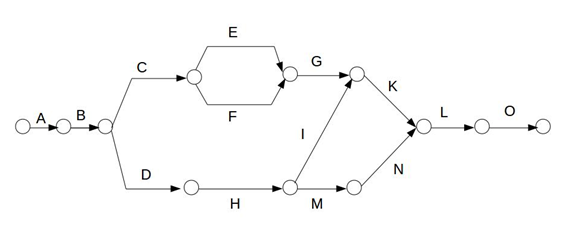
\includegraphics[scale=0.7]{QT2.png}
\end{center}
\end{figure}
\end{frame}
\subsection{Activities Sequencing}
\begin{frame}{Activities Sequencing}
\begin{itemize}
\item \textbf{Time Planning}
\item \textbf{Cost}
\end{itemize}
\end{frame}
\section{Executing and Monitoring}
\begin{frame}{Executing and Monitoring}
\begin{itemize}
\item \textbf{Quality Planning}
\item \textbf{Communication Planning}
\begin{itemize}
\item Metting
\item Gửi mail
\end{itemize}
\item \textbf{Human Planning}
\end{itemize}
\end{frame}
\end{document}
